\documentclass[12pt,a4paper]{article}

% -------------------
% MARK: Packages
% -------------------

% import geometry package to update the document margins
\usepackage[margin=1in]{geometry}
% set the font to helvectica
\usepackage[scaled]{helvet}
\renewcommand\familydefault{\sfdefault}
% for type-setting
\usepackage{amsmath, amssymb, amsfonts, verbatim, pifont}
% for slashed out text
\usepackage[normalem]{ulem}
% for units and scientific notation
\usepackage[table]{xcolor}
\usepackage{siunitx}
% for references and URLs
\usepackage{hyperref, url}
% Natbib setup for author-year style
\usepackage{natbib}
 \bibpunct[, ]{(}{)}{,}{a}{}{,}%
 \def\bibfont{\small}%
 \def\bibsep{\smallskipamount}%
 \def\bibhang{24pt}%
 \def\newblock{\ }%
 \def\BIBand{and}%
% for graphics and figures
\usepackage{graphicx, subfig, tikz}
% force figures to stay in their sections
\usepackage[section]{placeins}
% for tables
\usepackage{booktabs, longtable, tabularx}
\usepackage{multicol, multirow}
\usepackage{adjustbox}
\usepackage[flushleft]{threeparttable}
% a package for working with .csv data for tables
\usepackage{csvsimple}
% setup the algorithm package
% ruled: show bars around title and bar at bottom
% lined: show the line column on the left of the algorithm
% linesnumbered: print line numbers for each line
\usepackage[ruled,lined,linesnumbered]{algorithm2e}
\DontPrintSemicolon % don't print the semicolon that \; usually prints
% fix overfull hbox errors from oddities like using
% quotes (``foo'') and etc.
\usepackage{microtype}

% -------------------
% MARK: Debugging Packages
% -------------------

% import a debugging package to show the margin boxes
% \usepackage{showframe}

% -------------------
% MARK: Declarations
% -------------------

% setup captions for tables and figures
\captionsetup[table]{%
  labelfont={bf},
  name={Table},
  labelsep=colon,
  justification=raggedright,
  singlelinecheck=false}
\captionsetup[figure]{%
  labelfont={bf},
  name={Figure},
  labelsep=colon,
  justification=raggedright,
  singlelinecheck=false}
\captionsetup[algorithm2e]{%
  labelfont={bf},
  name={Figure},
  labelsep=colon,
  justification=raggedright,
  singlelinecheck=false}

% set the graphics path to the img directory
\graphicspath{{img/}}

% -----------------------------------------------------------------------------
% MARK: algorithm2e stuff
% -----------------------------------------------------------------------------

% params
% \SetKwInOut{Objects}{$\CKmatrix{O}$}
% \SetKwInOut{Weights}{$\CKvector{w}$}

% -------------------
% MARK: Headers
% -------------------

% headers and footers
\usepackage{fancyhdr}
\setlength{\headheight}{15pt}
\pagestyle{fancy}
\lhead{KautenjaDSP}
\rhead{\itshape FME7 v1.3.1}
\cfoot{\thepage}

% start the document
\begin{document}

% -------------------
% MARK: Title Page
% -------------------

% fancyhdr directive to remove headers from this title page
\thispagestyle{empty}
% center the title page contents
\vspace*{\fill}
\begin{center}

\includegraphics{FME7-Logo}
\linebreak\linebreak\linebreak\linebreak
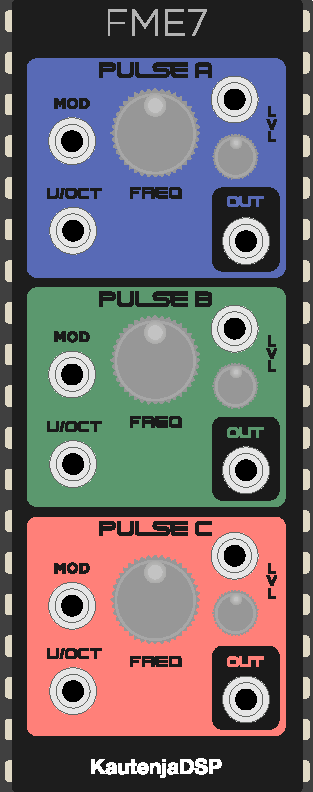
\includegraphics{FME7-Module}
\linebreak\linebreak\linebreak\linebreak

\includegraphics{KautenjaDSP}
\end{center}
\vspace*{\fill}
\clearpage

% -------------------
% MARK: Overview
% -------------------

\section{Overview}

FME7 is an emulation of the SunSoft FME7 (5B) sound chip from the Nintendo Entertainment System (NES) for VCV Rack. The FME7 chip contains three pulse wave generators with level control.

FME7 provides the key features of the FME7 chip, namely,
\begin{itemize}
  \item \textbf{Triple pulse wave generator:} Triple 12-bit pulse waves with duty cycle of $50\%$
  \item \textbf{Amplitude modulation:} Manual and CV control over the individual voice levels
\end{itemize}

% -------------------
% MARK: Panel Layout
% -------------------

\section{Panel Layout}

\begin{center}
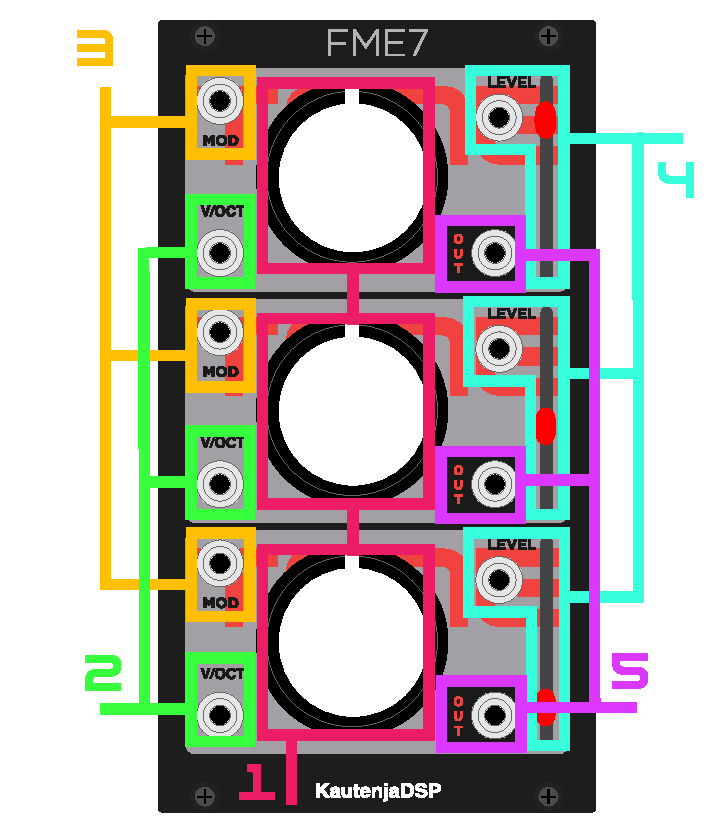
\includegraphics{FME7-Manual}
\end{center}

\begin{enumerate}
  \item Coarse frequency control for the pulse A, B, and C waveform generators.
  \item $V$/Octave inputs for pulse A, B, and C waveform generators.
  \item linear CV frequency modulation for pulse A, B, and C waveform generators.
  \item Level control for pulse A, B, and C waveform generators. When no CV is connected, the knob controls the level from $0\%$ to $100\%$. When a CV is connected, the knob acts as an attenuator.
  \item Channel outputs, ${\approx}10V_{pp}$.
\end{enumerate}

% -------------------
% MARK: References
% -------------------

\clearpage
\renewcommand\refname{References \& Acknowledgments}
\nocite{*}
\bibliographystyle{apalike}
\bibliography{references}

\end{document}
